\documentclass{standalone}
\usepackage{pgfplots}
\usepackage{tikz}

\begin{document}

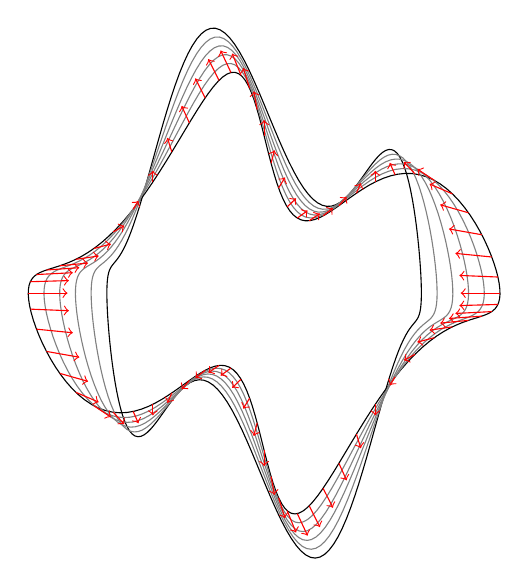
\begin{tikzpicture}
  \begin{axis}[axis lines=none, axis equal,
    width=1\textwidth,
    xmin=4,xmax=10,
    ymin=-4,ymax=4,
    ]
    \addplot[domain=0:360,samples=200]({7 +
      (1-cos(x*2)/2)*1.8*sin(x)},{(1-sin(x*4)/2)*1.8*cos(x)});

    \addplot[domain=0:360,samples=200]({7 +
      (1-0*cos(x*2)/2)*1.8*sin(x)},{1.2*(1-sin(x*4)/2)*1.8*cos(x)});

    \foreach \t in {1,...,4}
    \addplot[gray, domain=0:360,samples=200]
    ({7 + (1-(1-\t /5)*cos(x*2)/2)*1.8*sin(x)},
    {(1 + \t /25)*(1-sin(x*4)/2)*1.8*cos(x)});

    \foreach \q in {1,...,72}
    \addplot[->, red, domain=0:2.5,samples=5]
    ({7 + (1-(1-x /5)*cos(\q *5*2)/2)*1.8*sin(\q *5)},
    {(1 + x /25)*(1-sin(\q *5*4)/2)*1.8*cos(\q *5)});
  \end{axis}
\end{tikzpicture}

\end{document}


